%
% graphisch4.tex
%
% (c) 2020 Prof Dr Andreas Müller, Hochschule Rapperswil
%
\begin{figure}
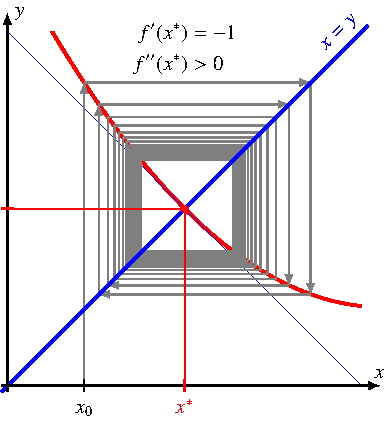
\includegraphics{chapters/10-arithmetik/figures/mnqp.pdf}
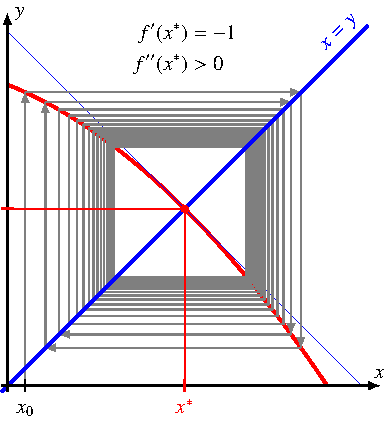
\includegraphics{chapters/10-arithmetik/figures/mnqn.pdf}
\caption{Die Fixpunktiteration $x_{n+1}=f(x_n)$ konvergiert sehr langsam
in der Umgebung des Fixpunktes $x^*$ für
$f'(x^*)=-1$ für $f''(x^*)\ne 0$.
\label{buch:figure:fixpunkt:ablm1}}
\end{figure}
